
\section{Evaluation}
\label{sec:5_eval}
% approx. 400-800 words
% \begin{itemize}
%     \item \textit{The metrics you used}
%     \item \textit{Results on evaluation that you performed}
%     \item \textit{Comparison and differences between you model and the baseline}
%     \item \textit{Correct interpretation of errors and analysis}
% \end{itemize}
\subsection{Metrics}
In this work we are framing the learning problem as a multi-class classification problem, where the classes to predict are the words in the vocabulary. Hence, we are training the model to minimize the cross-entropy (CE) loss:
\begin{equation}
    \text{CE} \parenth[\big]{f(x; \theta), y} = -\sum_{i=1}^{N} y_i \log{f(x_i; \theta)}
\end{equation}
% where $f(x; \theta)$ is the model, $x$ is the input sequence, $y$ is the target sequence, $\theta$ is the set of model parameters and $N$ is the number of classes in the vocabulary. 

The main metric we use to compare and evaluate the models is the \emph{perplexity} (PP). The reason is that PP is a well understood and established metric and it correlates well enough with the model performances on real-world tasks. Although the PP can be defined in multiple ways, it is convenient to use the definition of PP as the exponential of the cross-entropy (CE):
\begin{equation}
    \text{PP}(f(x; \theta), y) = \exp \parenth[\big]{CE(f(x; \theta), y)}
\end{equation}

% Intuitively, the PP can be interpreted as the number of classes that the model is considering to make a prediction . 
While the $CE$ gives a measure of how much the model is uncertain about the prediction, the PP can be interpreted as a measure of how many classes the model is considering to make a prediction (\emph{weighted branching factor}). The lower the PP, the less uncertain the model is on which word to predict, the better it is performing.

Additionally, we are further evaluating the best-performing model to excerpt deeper insights in its behaviour. Specifically, we are considering \emph{average PP per sequence length}, \emph{per word predicted vs. target counts difference} and \emph{F1 score}. Lastly, we are giving a qualitative evaluation of the model by showing some examples of generated sequences.

\subsection{Results}
We evaluated every model by performing an evaluation epoch on the \emph{validation} and \emph{test} set with batch size $1$. The results of these evaluation runs are summarized in Tab.\ref{tab:results}.
\begin{table}
    \begin{tabular}{lcc}
    \toprule
    \textbf{Model}& \textbf{Validation} & \textbf{Test} \\
    \midrule
    \texttt{baseline\_dropout} & 116.11 & 113.44 \\
    \texttt{merity\_ad} & 95.36 & 	91.29 \\
    \texttt{merity\_ad\_nohh} & 95.36 & 91.29 \\
    \texttt{merity\_ad\_nohh\_tbptt} & 90.38 &	87.46 \\
    \texttt{merity\_ad\_nohh\_1024} & 85.85 &	82.74 \\
    \texttt{merity\_ad\_nohh\_1024\_ps} & 87.40 &	83.18 \\
    \texttt{merity\_ad\_nohh\_1024\_ps\_long} & 83.01 &	79.86 \\
    \bottomrule
\end{tabular}
    \caption{Results (PP) of the experiments.}
    \label{tab:results}
\end{table}
It is worth noting that we decided to scrap \emph{Weight Dropout} on the hidden-to-hidden weight matrices of the LSTM layers. The reason is that the the model with the three dropout techniques (\texttt{merity\_ad}) was achieving worse results than the model with only \emph{Variational Dropout} and \emph{Embedding Dropout} (\texttt{merity\_eld}), as it can be seen in Fig.\ref{fig:tl_merity_ads}.

% \begin{figure}[h!]
%     \centering
%     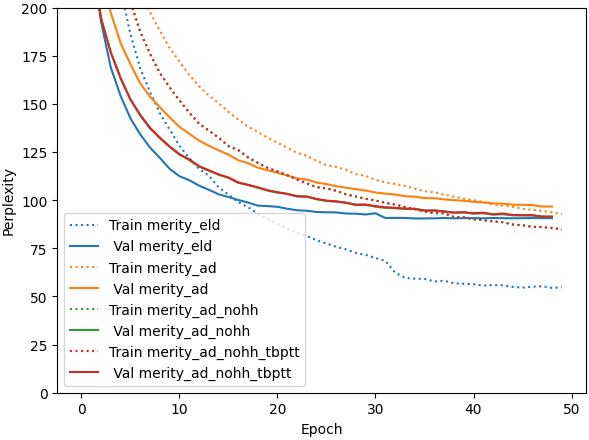
\includegraphics[width=.35\textwidth]{./assets/images/tl_merity_ads}
%     \caption{
%         Training and validation  PP of the models with dombined dropout techniques. %The \texttt{merity\_eld} model uses only \emph{Variational Dropout} and \emph{Embedding Dropout}, the \texttt{merity\_ad} model uses all the three dropout techniques and \texttt{merity\_ad\_nohh} removes dropout on the hidden-to-hidden weight matrices in \emph{Weight Dropout}.
%         }
%     \label{fig:tl_merity_ads}
% \end{figure}

\begin{figure*}

    \floatsetup{floatrowsep=Qquad}
    \begin{floatrow}
        
      \ffigbox[\FBwidth]{
        \caption{
        Train and valid PP of the models with combined dropout techniques. %The \texttt{merity\_eld} model uses only \emph{Variational Dropout} and \emph{Embedding Dropout}, the \texttt{merity\_ad} model uses all the three dropout techniques and \texttt{merity\_ad\_nohh} removes dropout on the hidden-to-hidden weight matrices in \emph{Weight Dropout}.
        }
        \label{fig:tl_merity_ads}}
        {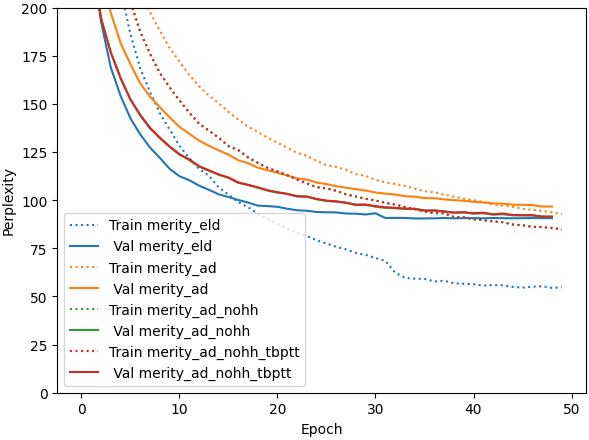
\includegraphics[width=.3\textwidth]{./assets/images/tl_merity_ads}}

    \ffigbox[\FBwidth]{
        \caption{Ablation study on \texttt{merity\_wd}.}
        \label{fig:tl_merity_wd}}
        {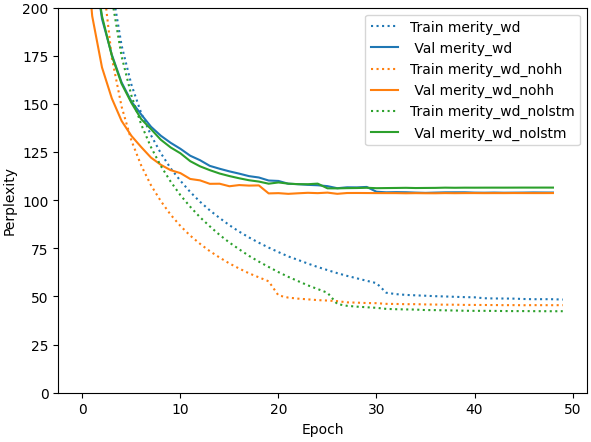
\includegraphics[width=.3\textwidth]{./assets/images/tl_merity_wd}}\hskip2em

    \ffigbox[\FBwidth]{
        \caption{Impact of larger model size and partial shuffle.}
        \label{fig:tl_merity_1024_ps}}
        {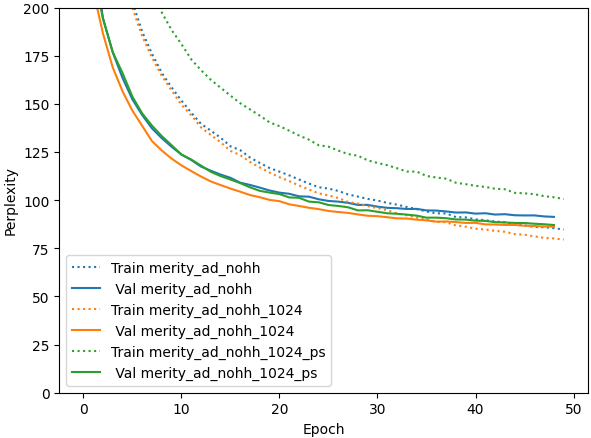
\includegraphics[width=.3\textwidth]{./assets/images/tl_merity_1024_ps}}
    \end{floatrow}
\end{figure*}

Hence, we performed further experiments on the \texttt{merity\_wd} model. We found out that \texttt{merity\_wd\_nohh} was achieveng better results on the validation set, as in Fig\ref{fig:tl_merity_wd}. This behaviour is probably caused by the fact that dropping out the hidden-to-hidden weights prevents the model from effectively learn long-term dependencies in the sequences. In the end, we decided to keep the \texttt{merity\_ad\_nohh} model as it had the best performances and still little overfitting.
% \begin{figure}[h!]
%     \centering
%     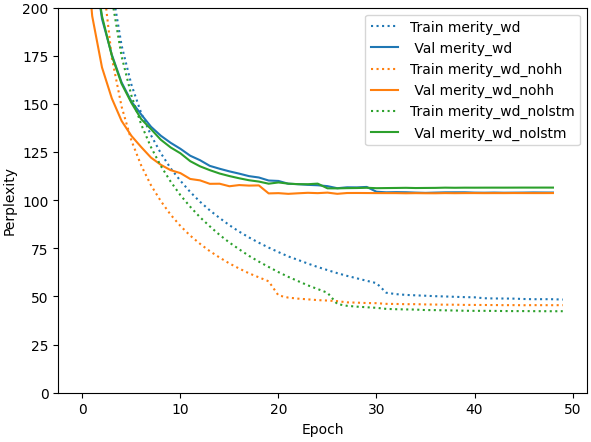
\includegraphics[width=.35\textwidth]{./assets/images/tl_merity_wd}
%     \caption{Ablation study on \texttt{merity\_wd}.}
%     \label{fig:tl_merity_wd}
% \end{figure}

For similar reason we decided to discard TBPTT as training algorithm, as it was not improving the performances, and stick with unconstrained BPTT. On the other end, the models with increased embedding and hidden sizes achieved better results; we also reduced the number of LSTM layers from $3$ to $2$ and increased the probabilities of the dropout techniques to account for the increased model size. Similar considerations hold for the usage of \emph{Partial Shuffle}, which ensures less overfitting at the expensive of slightly higher PPs; the reason is that partially shuffling the sentences increases variety in the training data, acting as a sort of data augmentation technique. Lastly, we performed an extensive training experiment on the \texttt{merity\_ad\_nohh\_1024\_ps} model, where we let it train until the validation loss would stop decreasing at epoch $96$; this final and best performing model model scored $83.01$ PP on the validation set and $79.86$ on the test set.

\subsection{Analysis}
This section is dedicated to the analysis of the best performing model, \texttt{merity\_ad\_nohh\_1024\_ps\_long}. We start by providing some examples of generated sequences\footnote{In order to try and use the model, we recommend to use the  TUI application in the repository attached to this work.}, in the format: \texttt{<prompt>} (\textless temperature \textgreater) $\rightarrow$ \textless inferred \textgreater:
\begin{itemize}
    \item \texttt{the} ($1.0$) $\rightarrow$ the major \texttt{<unk>} million foreign equipment received a \$ N million offer for federated and packaged goods companies;
    \item \texttt{the price} ($0.8$) $\rightarrow$ the price for the giant company is about \$ N million;
    \item \texttt{the price} ($1.0$) $\rightarrow$ the price advanced increase in the second quarter in workstations prompting the dollar to a steep rise in the week 's sharp climb in the imports growth of the;
\end{itemize}

We can see that the model is able to generate sequences that are roughly syntactically correct. However, the generated sequences are not semantically solid. This is probably due to the fact that the model is not able to learn the meaning of the words, but only their distribution in the sequences. Moreover, it seems that the model has consistent performances on shorter sequences and that it struggles more on longer sequences. This is also visible on the average PP per sequence length, as in Fig.\ref{fig:avg_pp_per_seq_len}: sentences of length shorter than $40$ tokens cause the model to score $60 \le PP \le 100$, slightly increasing as the length decreases. On the other hand, sentences of length longer than $40$ tokens have PP scores as high as $160$ and as low as $20$.
\begin{figure}[htb]
    \centering
    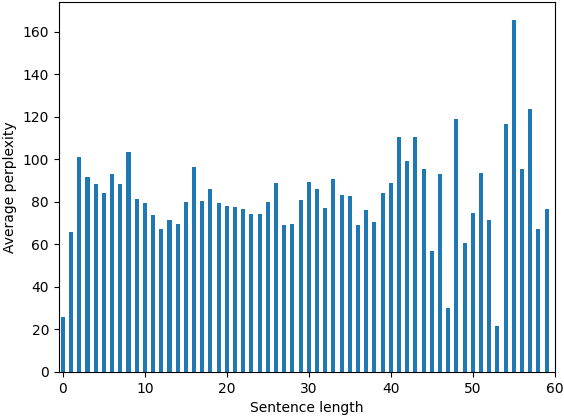
\includegraphics[width=.815\textwidth]{./assets/images/ppl_by_len}
    \caption{Average PP per sequence length.}
    \label{fig:avg_pp_per_seq_len}
\end{figure}

If we inspect the counts of predicted and target words in Tab.\ref{tab:diff_counts}, we can see that the model heavily relies on the most present words in the dataset: the 5 most guessed words make up over $50\%$ of the total predictions, while the 5 most present words in the target sequences make up only $20\%$ of the total target words. All of the 10 most guessed words are over-represented in the predictions, except \texttt{and} - roughly on par - and \texttt{in} - which shows a slightly negative difference. Quite interestingly, the fact that the \texttt{<eos>} token is over-represented may indicate that the model has not learned when it is most appropriate to terminate a sentence. 

\begin{table}[hbt]
    \centering
    \begin{tabular}{lcccccc}
\hline
\textbf{} & \textbf{word} & \textbf{target\_count} & \textbf{target\_freq} & \textbf{pred\_count} & \textbf{diff} & \textbf{pred\_freq} \\
\hline
0 & \textless unk\textgreater & 4606 & 5.85\% & 15026 & 10420 & 19.10\% \\
\hline
1 & the & 3968 & 5.04\% & 12405 & 8437 & 15.77\% \\
\hline
2 & \textless eos\textgreater & 3761 & 4.78\% & 9125 & 5364 & 11.60\% \\
\hline
3 & N & 2494 & 3.17\% & 3874 & 1380 & 4.92\% \\
\hline
4 & of & 2182 & 2.77\% & 3236 & 1054 & 4.11\% \\
\hline
5 & to & 2024 & 2.57\% & 2878 & 854 & 3.66\% \\
\hline
6 & a & 1739 & 2.21\% & 2315 & 576 & 2.94\% \\
\hline
7 & and & 1471 & 1.87\% & 1480 & 9 & 1.88\% \\
\hline
8 & in & 1470 & 1.87\% & 1366 & -104 & 1.74\% \\
\hline
9 & 's & 903 & 1.15\% & 1341 & 438 & 1.70\% \\
\hline
\end{tabular}
    \caption{Per word predicted vs. target counts difference.}
    \label{tab:diff_counts}
\end{table}

Finally, we can get some interesting insights by looking at the f1-score in Tab.\ref{tab:f1}. Quite expectedly, given the huge size of the targets space and the nature of the task of language modelling, most of the classes have a rather low f1-score; this is particularly noticeable in the most common words, like \texttt{<unk>} ($0.23$) and \texttt{the} ($0.34$). However, it is interesting to notate than some very specific words score higher values. If we take a look at the words with highest f1-score with support $\ge 100$, we can see interesting examples like \texttt{million} ($0.68$) and \texttt{N} ($0.62$), which may indicate that the model was effective in learning where to place numbers and to phrase them together. Scores can get even higher if we reduce the support threshold to $\ge 10$: words that may appear in very specific phrasings show pretty interesting scores (\texttt{angeles} ($0.95$), \texttt{share} ($0.8$), \texttt{estate} ($0.79$)).

\begin{table}[hbt]
    \centering
    \begin{tabular}{lll}
    \toprule
    \textbf{support} $\ge 100$ &\textbf{support} $\ge 10$ & \textbf{full support}  \\
    \midrule
    hutton 1.0 & share 0.8& \textless eos \textgreater 0.4\\
    kong 1.0 &million 0.68& on 0.22\\
    lehman 0.95 & N 0.62& \textless unk \textgreater 0.23\\
    angeles 0.95 & than 0.55 & N 0.62 \\
    lynch 0.89 & co. 0.54 & the 0.34 \\
    officer 0.84 & billion 0.51 & \$ 0.45 \\
    share 0.8 & year 0.51 & as 0.31 \\
    estate 0.79 & president 0.51 & a 0.23 \\
    loan 0.79 & n't 0.49 &  is 0.17\\
    cents 0.78& of 0.46  & of 0.46 \\
    \bottomrule
\end{tabular}



    \caption{predicted words ranked by F1 score with various filters on support.}
    \label{tab:f1}
\end{table}
